\section{Dataset Collection}

We use the Stack Exchange Data
Explorer\footnote{\texttt{https://data.stackexchange.com/stackoverflow/query/new}}
and construct a custom SQL query on the Stack Overflow data. The query could be
found under \texttt{source\_code/query.sql}.

The query satisfies the three requirements:

\begin{itemize}
    \item \texttt{\ldots select top 500} means that we are collecting at least
    500 threads.
    \item \texttt{\ldots Tags like \textquotesingle{}\%python\%\textquotesingle{}}
    means that we are collecting threads tagged \texttt{python}, discussing the
    Python programming language.
    \item \texttt{\ldots where AnswerCount >= 1} means we are collecting
    threads with at least 1 question and 1 answer.
\end{itemize}

The dataset contains 500 questions and 1254 answers, an average of 2.508 answers
per question. The distribution of answers is shown in Figure~\ref{ans-dist}.

\begin{figure}[h]
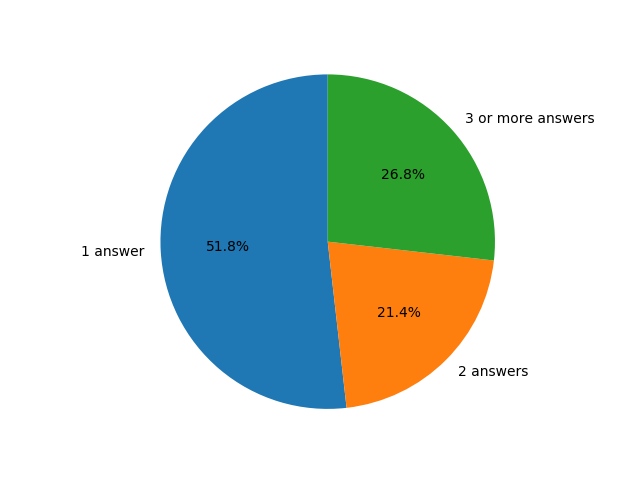
\includegraphics[width=0.9\linewidth]{no_ans_per_qn}
\caption{Distribution of answers}\label{ans-dist}
\end{figure}

\section{Dataset Analysis and Annotation}

\subsection{Stemming}

We used NLTK~\cite{nltk} to process the dataset.

\subsection{POS Tagging}

We picked 10 sentences at random and applied POS tagging, using NLTK\@.
The results are as follows:

\begin{table}
\caption{POS Tagging}
\begin{tabu}{X[1.15,l]X[2,l]}
    \textbf{Sentence} & \textbf{POS Tagging} \\
    \midrule
    You are being tricked by Python's representation of the result string.&
    (You,PRP), (are,VBP), (being,VBG), (tricked,VBN), (by,IN), (Python,NNP),
    ('s,POS), (representation,NN), (of,IN), (the,DT), (result,NN), 
    (string,NN), (.,.) \\
    I like this rough, succinct definition: A function that can refer to 
    environments that are no longer active.&
    (I,PRP), (like,VBP), (this,DT), (rough,NN), (,,,), (succinct,JJ),
    (definition,NN), (:,:), (A,DT), (function,NN), (that,WDT), (can,MD),
    (refer,VB), (to,TO), (environments,NNS), (that,WDT), (are,VBP), (no,DT),
    (longer,RBR), (active,JJ), (.,.) \\
    Isn't that what Anders' second example does? &
    (Is,VBZ), (n't,RB), (that,IN), (what,WP), (Anders,NNP), (',POS),
    (second,JJ), (example,NN), (does,VBZ), (?,.) \\
    There's nothing that will automatically do what you want. & 
    (There,EX), ('s,VBZ), (nothing,NN), (that,WDT), (will,MD),
    (automatically,RB), (do,VB), (what,WP), (you,PRP), (want,VBP), (.,.) \\
    Use a subrange of [\textbackslash{}u0000-\textbackslash{}uFFFF] for what
    you want. &
    (Use,VB), (a,DT), (subrange,NN), (of,IN), ([,JJ),
    (\textbackslash{}u0000-\textbackslash{}uFFFF,JJ), (],NN),
    (for,IN), (what,WP), (you,PRP), (want,VBP), (.,.) \\
    Tom says it all really. &
    (Tom,NNP), (says,VBZ), (it,PRP), (all,DT), (really,RB), (.,.) \\
    I have been sold on mod\_wsgi and apache rather than in mod\_python. &
    (I,PRP), (have,VBP), (been,VBN), (sold,VBN), (on,IN), (mod\_wsgi,NN),
    (and,CC), (apache,NN), (rather,RB), (than,IN), (mod\_python,NNS), (.,.) \\
    This topic is covered in Django tutorials. &
    (This,DT), (topic,NN), (is,VBZ), (covered,VBN), (in,IN), (Django,NNP),
    (tutorials,NNS), (.,.) \\
    The single * means that there can be any number of extra positional
    arguments. &
    (The,DT), (single,JJ), (*,NN), (means,VBZ), (that,IN), (there,EX), (can,MD),
    (be,VB), (any,DT), (number,NN), (of,IN), (extra,JJ), (positional,JJ),
    (arguments,NNS), (.,.) \\
\end{tabu} 
\end{table}

\subsection{Token Definition and Annotation}

\section{Tokenizer}

\section{Further Analysis and Annotation}

\section{Application}